\section{Galois Field}
Galois fields are the finite fields. ``They can be completely characterized in terms of splitting fields of some polynomials. It is found that the Galois group of an extension of a finite field by a finite field is cyclic'' \cite{hunger}. We denote Galois field with \(q\) elements by \(GF(q)\).

\begin{definition} \cite{hunger} [Prime Fields]
Let \(F\) be a field and let \(P\) be the intersection of all subfields of \(F\). Then \(P\) is a field with no proper subfields. This field \(P\) is called the Prime subfield of \(F\).
\end{definition}

\begin{enumerate}
\item ``If \(charF=p(prime)\), then \(P\cong {\mathbb{Z}}_p\).
\item If \(charF=0\), then \(P\cong \mathbb{Q}\)'' \cite{hunger}.
\end{enumerate}

\begin{theorem} \cite{hunger}
A  finite field \(F\) has \(p^n\) number of elements where \(p \in \mathbb{Z}_+\) is a prime and it has \(p^n\) number of elements if and only if \(F\) is a splitting field of \(x^{p^n} - x\) over \(\mathbb{Z}_p\).
\end{theorem}
\vspace{4mm}

\begin{theorem} \cite{hunger}
  If \(F\) is a finite dimensional extension field of a finite field \(K\), then \(F\) is finite and is Galois over \(K\). The Galois group \(Aut_K^F\) is cyclic.
\end{theorem}
\clearpage

\section{Representation of Galois Fields}
Basically there are two types of representation of a finite field. These two representations are equivalent.
\subsection{Integer representation}

``\(GF(p^n)=\{0,1,...,p-1\} \cup \{p,p+1,...,p+p-1\} \cup ... \cup \{p^{n-1},p^{n-1}+1,...,p^{n-1}+p^{n-2}+...+p-1\}\)'' \cite{galois}.

\begin{example}
    \(GF(2)=\{0,1\}\)\\
    \(GF(2^3)=\{0,1\} \cup \{2,2+1\} \cup \{2^2,2^2+1,2^2+2,2^2+2+1\}=\{0,1,2,3,4,5,6,7\}\)
\end{example}

But the digits \(2,3,..,7\) of the field \(GF(2^3)\) do not lie on the field \(GF(2)\). If we look the field \(GF(2^3)\) as an extension field of \(GF(2)\) and write its elements using only the elements of the base field \(GF(2)\) then we have the following representations:
\vspace{3mm}

\begin{table}[h!]
  \centering
\begin{tabular}{|c|c|c|}
    \hline
    Digits & Expansion & Binary rep..\\
    \hline
    3 & \(2+1\) & 011 \\
    4 & \(2^2+2^1 \times 0 +2^0 \times 0\) & 100 \\
    5 & \(2^2+1\) & 110 \\
    \hline
\end{tabular}
\caption{\small Binary representation table of field elements.}
\end{table}
\vspace{3mm}

This is actually \textbf{Binary representation} of the field \(GF(2^3)\)



\subsection{Polynomial representation}
``For a field \(F\) and an irreducible polynomial \(f(x) \in F[x]\) the quotient ring \(F[x]/(f(x))\) is field'' \cite{galois}.\\
If \(F\) is a finite field consisting of \(p\) elements and \(f(x) \in F[x]\) is irreducible then \(F[x]/(f(x))\) is finite field. This field consists of all polynomials modulo \(f(x)\). If \(F=GF(2^3)\) then \(f(x)= x^8+x^7+...+x+1 \in F[x]\) is irreducible in \(F[x]\). Since \(F\) has \(8\) elements which are modulo \(8\), elements of \(F\) is represented by the elements of the factor ring \(F[x]/(f(x))\) \cite{aes}. \\


In the example-5, the number \(5\) has the representation \(2^2+1\). This gives the polynomial representation \(x^2+1=(1,0,1)\)(coefficient of \(x^2\) is \(1\) of \(x\) is \(0\) and of constant is \(1\) ) Now the binary equivalent of \(5\) is \(101\).

\subsection{Operations in Galois Field}
Let the Galois field be \(GF(p^n)\). Since the elements of a Galois field can be represented as polynomials the operations are similar to polynomial operations. Let \(f(x)=a_0+a_1x+..+a_{n-1}x^{n-1}\) and \(g(x)=(b_0+b_1x+...+b_{n-1}x^{n-1}\).
\begin{enumerate}
  \item Addition \\
  \(f(x)+g(x)\;\;\;\; (modp)\)
  \item Multiplication \\
  \(f(x).g(x)\;\;\; (modp)\) \cite{aes}.
\end{enumerate}

\section{Error-Correcting Code}
The loss of information is inevitable. It cannot be prevented or stopped. So, we need a way of retrieving the lost information or correcting the false information.

\begin{enumerate}
\item Paintings gets deteriorated over time and has to be renovated.
\item The data stored in a CD is lost over time \cite{coding}.
\end{enumerate}

To be able to detect and correct errors during transmission of information in digital system "coding theory" is developed. The idea of coding theory is to append some extra digits to the information and use this to detect and possibly correct the errors during transmission.
\begin{definition} \cite{coding}
  These codes that can correct themselves are called ``Error correcting codes''
\end{definition}
In digital system, information are transmitted as strings of \(0\) and \(1\). So the fundamental of the coding theory in computer system is the manipulation of strings of binary digits. The proper and complete manipulation of these strings is possibly only if the space of the strings is a field. This field is finite so this field is a \textbf{Galois field}. This is where the application of Galois theory comes.
Another advantage of using field is that the space of code forms a vector space over the base field. \\
The widely used field for coding in electronically transmitting device is an extension field \({\mathbb{Z}}_2\) which is the field \(GF(2)\) consisting of \(0\) and \(1\). Recent works has shown that it is possible to extend codes to more general type of numbers called rings. This rings are called "Galois rings" \cite{error_correct}.\\

The non-empty set of symbols for the code \(\mathcal{A}\) called \textbf{alphabet}. A finite sequence of elements from \(\mathcal{A}\) is called a \textbf{word} over \(\mathcal{A}\). Let \(\mathcal{A}^*\) be the set of all words over \(\mathcal{A}\). A subset \(C\) of \(\mathcal{A}\) is called a code.
If the cardinality of the alphabet \(\mathcal{A}\) is \(q\) then the code \(C\) is called \(q-ary code\). For \(q=2\) it is called binary and for \(q=3\) it is called terniary \cite{error_correct}.

\subsection{Linear Codes}
Let \(K=GF(q)\) be a Galois field. Then a finite extension of \(K\) of dimension \(n\) is \(V=GF(q)^n=GF(q^n)\).
\begin{definition} \cite{coding}
  A linear code \(C\) is a subspace of \(V\). \\
  The code \(C\) has dimension \(k \leq n\) and the length \(n\). It is called a ``\((n,k)\) code'' \cite{error_correct}.
\end{definition}

The usefulness of linear code is that they are vector spaces over the base field so they have a basis. All the code words can be generated with this basis. Instead of storing all \(2^k\) number of code words (for \(k\)-dimensional binary codes), storing only \(k\) basis elements is sufficient which saves massive storage.\\[2mm]
Let \(C\) be \((n,k)\) code which is a subspace of \(V\).

\begin{definition} \cite{error_correct} [Generator Matrix]
  Let \(\{v_1, v_2,...,v_k\}\) be a basis of \(C\). A generator matrix is the \(k \times n\)
  \[G=\begin{pmatrix}
      v_1\\
      v_2\\
      .\\
      .\\
      .\\
      v_k
    \end{pmatrix}
  \]
\end{definition}
\vspace{2mm}

\begin{definition} \cite{error_correct} [Parity check matrix]
  ``The dual code of \(C\) is the set \(C^{\perp}=\{x \in V \;| \; x.y=0 \;\; \forall y \in V \}\). The dual code is a code in itself and has dimension \(n-k\).\\
  The \(C^{\perp}\) is linear so it has a generator matrix. ``A generator matrix \(H\) of \(C^{\perp}\) is called a parity check matrix'' \cite{error_correct}.
\end{definition}

\begin{theorem} \cite{coding}
  If \(G=(I_{k \times k},A_{k \times (n-k)})\) is a generator matrix of an \((n,k)\) code \(C\) then its parity check matrix is \(H=(I_{(n-k) \times (n-k)}, A'\) where \(A'\) is the transpose of \(A\).
\end{theorem}

\begin{definition} \cite{coding}
  The \textit{Hamming distance} between \(v,w \in V\) is defined by \(d_h(v,w)=|\{i\;|\; v_i \neq w_i;\; 1 \leq i \leq n \}|\).\\
  The \textit{minimum distance} of a code \(C\) is defined as \(min\{d_h(v,w)\;|\; d_h(v,w) \neq 0, v,w \in C\}\).\\
  ``The weight of a vector is its distance from zero and the \textit{minimum weight} of a code \(C\) is the minimum weight of all non-zero weights of the vectors in \(C\)'' \cite{error_correct}.
\end{definition}

\begin{theorem} \cite{error_correct}
  A linear code \(C\) with minimum weight \(d\) can correct strings having number of errors up to \(t= \lfloor (d-1)/2 \rfloor\).
\end{theorem}

\subsection{Illustration}
To apply \((n,k)\) coding first we need to group our information into blocks of length \(k\).
\(u_1,...,u_k\),  \(u_k,...,u_{2k}\),... . This space has dimension \(k\). Now these block of codes are encoded separately each to a code of length \(n\) as shown \cite{coding}.

\vspace{5mm}
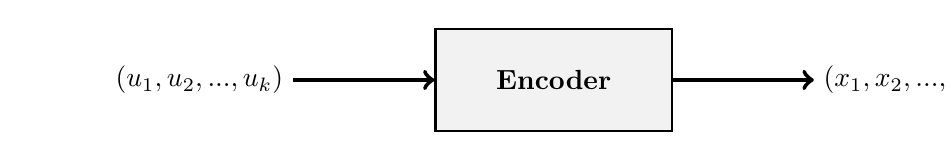
\begin{tikzpicture}
  \hspace{1cm}
  \node [] (u) {\((u_1,u_2,...,u_k\))};
  \node[
  right of=u,
  rectangle,
  draw,
  thick,
  fill=gray!10,
  minimum width=30mm,
  minimum height=13mm,
  xshift=35mm] (e) {\bfseries Encoder};

  \node[right of=e, xshift=35mm] (x) {\((x_1,x_2,...,x_n)\)};

  \draw[->,ultra thick] (u)--(e);
  \draw[->,ultra thick] (e)--(x);
\end{tikzpicture}

\vspace{4mm}
\noindent
Mathematically, the encoded vector \(x\) is obtained form the original vector \(u\) using the generator matrix \(G\) by the relation \(x=uG\) \cite{coding}.\\[5mm] To continue and complete the diagram.\\

\vspace{4mm}
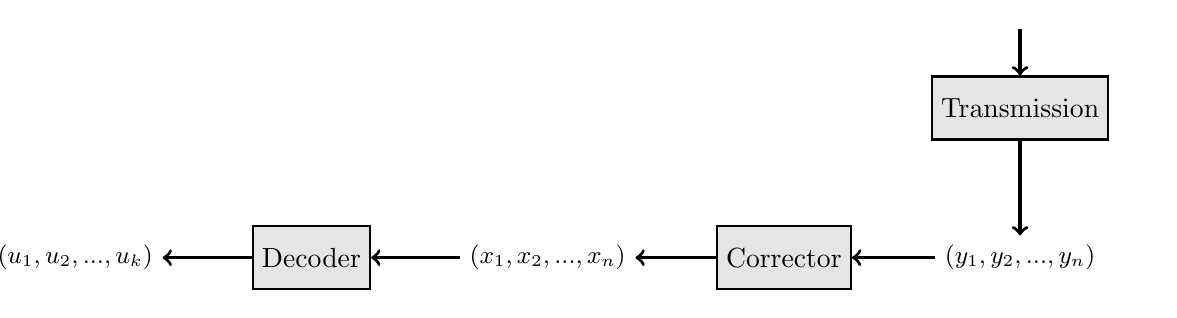
\begin{tikzpicture}
  \hspace{-5mm}
  \node[
  rectangle,
  draw,
  thick,
  fill=gray!20,
  minimum width=13mm,
  minimum height=8mm,
  ] (t) {Transmission};

  \node[below of=t, yshift=-9mm] (y) {\small \((y_1,y_2,...,y_n\))};

  \node[
  left of=y,
  rectangle,
  draw,
  thick,
  fill=gray!20,
  minimum width=13mm,
  minimum height=8mm,
  xshift=-20mm] (c) {Corrector};

  \node[left of=c, xshift=-20mm] (x) {\small \((x_1,x_2,...,x_n)\)};

  \node[
  left of=x,
  rectangle,
  draw,
  thick,
  fill=gray!20,
  minimum width=13mm,
  minimum height=8mm,
  xshift=-20mm] (d) {Decoder};

  \node[left of=d, xshift=-20mm] (u) {\small \((u_1,u_2,...,u_k\))};


  \draw[->,very thick] (0,1)--(t);
  \draw[->,very thick] (t)--(y);
  \draw[->,very thick] (y)--(c);
  \draw[->,very thick] (c)--(x);
  \draw[->,very thick] (x)--(d);
  \draw[->,very thick] (d)--(u);
\end{tikzpicture}

\vspace{9mm}
\section{Syndrome Decoding}
\begin{definition} \cite{error_correct}
  The syndrome of a vector \(y \in V\) is defined as \\ \(syn(y)=\begin{pmatrix}
    y.h_1\\
    y.h_2\\
    .\\
    .\\
    .\\
    y.h_{n-k}
  \end{pmatrix}\), \hspace{12mm} where \(\begin{pmatrix}
    h_1 \\ h_2\\ .\\ .\\ .\\ h_{n-k}
  \end{pmatrix}\) is the parity check matrix of \(C\).
\end{definition}
\vspace{3mm}
Now the code \(C\) is a subgroup of \(V\) under addition. Moreover, it is a normal subgroup of \(V\).
\begin{theorem} \cite{error_correct}
  Two vectors in \(V\) have the same syndrome if and only if they are in the same co-set of \(C\).
\end{theorem}

\subsection{Decoding Process}
Suppose the signal received is the vector \(y\).
\begin{enumerate}
\item First we determine its syndrome, \(syn(y)\).
\item Determine the co-set of \(C\) containing \(syn(y)\), say \(e + C\).
\item Then \(y=e+x\) for some \(x \in C\). This implies \(x=y-e\). Since \(x \in C\), this \(x\) is the required decoding of \(y\) \cite{error_correct}.
\end{enumerate}
This \(e\) is also called "error vector" \cite{error_correct}.
\vspace{2mm}

\begin{example}
  Consider a generator matrix \(G=\begin{pmatrix}
    1 & 0 & 1 & 0\\
    0 & 1 & 1 & 1
  \end{pmatrix}\). Then the parity check matrix is \(H=\begin{pmatrix}
    1 & 1 & 1 & 0\\
    0 & 1 & 0 & 1
  \end{pmatrix}\). And the code generated by \(G\) is  \(C=\{(0,0,0,0),(1,0,1,0),(0,1,1,1),(1,0,1,1)\} \;\; \subset GF(2^{4})\).\\

  Suppose the received vector is \(y=(1,1,1,0)\). Then \(y \not \in C\) so the information is distorted from the original information. To get the original information:\\
  \(syn(y)= \begin{pmatrix}
    y.h_1 \\ y.h_2
  \end{pmatrix} = \begin{pmatrix}
    1 \\ 1
  \end{pmatrix}\) where \(h_1\) is the first row and \(h_2\) is the second row of \(H\).\\
  Now if \(e=(0,1,0,0)\) then \(e+C=\begin{pmatrix}
    1 \\ 1
  \end{pmatrix}\) so \(y-e=(1,1,1,0)-(0,1,0,0)=(1,0,1,0) \in C\) is the original information \cite{error_correct}.

\end{example}


\subsection{Perfect Code}
The code \(C \subseteq V\) as of above is perfect if the union of all the spheres of radius \(t\) about its code-words is the vector space \(V\).\\
This code is \(C\) is called perfect because every received vector with the number of errors given by \(t\) can be decoded to a code-word of \(C\) \cite{error_correct}.

\begin{example}
  The code \(C=V\) is a perfect code. This code cannot correct any errors because every possible code word is in the \(C\). Therefore this perfect code is trivial \cite{error_correct}.
\end{example}

\begin{example}
  The general binary Hamming code \(H_r\), \(r \in \mathbb{N}\) whose parity check matrix \(H\) column consisting of non-zero r-tuples \cite{error_correct}.
\end{example}

\section{Cyclic Code}
The code \(C\) as of above is cyclic if \((a_0,a_1,...,a_{n-1}) \in C \implies (a_{n-1},a_0,...,a_{n-2}) \in C\).\\

Suppose \(C\) is a code over a Galois field \(F=GF(q)\). Then there exist a correspondence \(\Phi : C \mapsto F[x]/(x^n-1)\) such that \(\{(a_0,a_1,...,a_{n-1}),(a_1,...,a_{n-1},a_0),....,(a_{n-1},a_0,....,a_{n-2})\} \longmapsto a_0+a_1x+a_2x^2+...+a_{n-1}x^{n-1}\). \\

This map \(\Phi\) is homomorphism. This shows that the cyclic code \(C\) can be embedded into the ring \(R_n=F[x]/(x^n-1)\) \cite{error_correct}.
\vspace{5mm}
\begin{theorem} \cite{error_correct}
  \begin{enumerate}
  \item A subset \(S\) of \(R_n\) corresponds to a cyclic code if and only if \(S\) is an ideal of \(R_n\) and
  \item if \(S=(g(x))\) if and only if  \(g(x)\) divides \(x^n-1\).
  \end{enumerate}
\end{theorem}

\begin{tcolorbox}
  This theorem determines all cyclic codes. They are ideals of \(R_n\) and these ideals are generated by the polynomials that divides \(x^n-1\). Thus cyclic code have a generator polynomial which is computationally simpler than having a generator matrix. \\[2mm]
  This is where usages of polynomial representation of finite fields come into play and this is where cyclic code has advantage over general linear code.
\end{tcolorbox}

\vspace{5mm}
\begin{example}
  The divisors of \(x^3-1 \in F=GF(2^{3})\) are \(1, x+1, x^2+x+1, x^3-1\).\\
  For \(g(x)=x+1\) we have \(F[x]/(g(x))=\{(0),(1+x),(1+x^2),(x+x^2)\}\) so the corresponding cyclic code is \(\{(0,0,0),(1,1,0),(1,0,1),(0,1,1)\}\) \cite{error_correct}.
\end{example}

\vspace{7mm}
``Similar to general linear codes which are defined using the generator matrix or the parity-check matrix, cyclic codes are defined using generator polynomial or parity-check polynomial and the advantage of cyclic code is that there exists efficient algebraic decoding algorithm for them'' \cite{coding}.

\subsection{Usages}
\begin{enumerate}
\item The \((3,1)\) binary code is used in the short-range wireless communication system like \(Bluetooth^{TM}\) \cite{wireless}.
\item The Hamming Code \((7,4)\) is used in memory devices like RAM \cite{coding}.

  \item The Cyclic codes are used in storing data in CDs and DVDs \cite{coding}.
  \end{enumerate}
  \vspace{9mm}

  \begin{figure}[h]
    \centering
    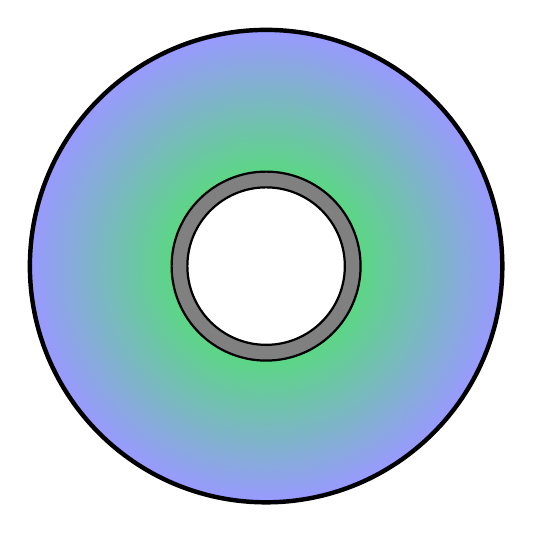
\begin{tikzpicture}
      \draw [ultra thick, outer color=blue!40, inner color= green!80] (0,0) circle [radius=3];
      \draw[thick, fill=gray] (0,0) circle [radius=1.2];
      \draw[thick, fill=white] (0,0) circle [radius=1];
    \end{tikzpicture}
    \caption*{\footnotesize A CD}
  \end{figure}



  \section{Cryptography}
It is the science of safe-guarding information by converting the original message into something unreadable.\\
Galois Fields are the life of modern cryptography used in digital communication.

\subsection{Advance Encryption Standard(AES)}
The Advance Encryption Standard is a Computer Security Standard for cryptography which is approved by the ``Federal Information Processing Standards Publications'' of USA which became effective on May 26, 2002. ``The AES algorithm is a \textit{symmetric block cipher} that can encrypt and decrypt digital information'' \cite{aes}. Symmetric key cryptography is used to share information between two parties where the two parties share a secret ``key'' and a public encryption algorithm.\\

``In 2000, National Institute of Standards and Technology(NIST) announced the selection of the ``Rijndael'' block cipher family as the winner of the AES competition and since then AES has been the standard for digital cryptography'' \cite{aes}. ``The Rijendael block cipher was developed by two Belgian cryptographers, \textbf{Vincent Rijmen and Joan Daemen}'' \cite{aes}.\\

The generic algorithm of AES consists of smaller sub-algorithms namely\\ ``Sub-Bytes, Shift-Rows, Mix-Columns and Add-Round-Key'' \cite{aes}.

\begin{table}[h!]
  \centering
\begin{tabular}{|l|l|}
  \hline
  Bit & \hspace{7mm}A binary digit: 0 or 1.\\
    \hline
  Byte & \hspace{7mm}A sequence of 8 bits.\\
    \hline
  Block & \hspace{7mm} A sequence of bits of a fixed length.\\
  \ & \hspace{13mm}In this Standard, block consists of 128 bits.\\
    \hline
  Block cipher &  \hspace{7mm} A family of permutations of blocks.\\
    \hline
  Key & \hspace{7mm}The parameter that selects the permutation\\
  \ & \hspace{13mm}from the block cipher.\\
    \hline
\end{tabular}
\caption{\small Terms and their meanings.}
\end{table}


\vspace{7mm}
\section{The Cipher(Algorithm)}
\subsection{The State}
First the data is broken into blocks and each block is broken into smaller chunks of a size byte (16 bytes for a block of size 128 bits). This block is then represented in a \(4 \times 4\) matrix whose each entry is a byte of the block. This matrix is called the State.\\
  Suppose the block is \(b_1, b_2,...,b_{16}\). Then the state is
    \(\left[\begin{smallmatrix}
  b_1 & b_5 &... & ...\\
  b_2 & b_6 &... & ...\\
  b_3 & b_7 &... & ...\\
  b_4 & b_8 &... & b_{16}
\end{smallmatrix}\right]\).\\[2mm]

Mathematical operations are not applicable to the data directly so the significance of this step is to make the data applicable for mathematical operations.\\
For the 128-bit key encryption the algorithm forms a \(4 \times 4\) matrix with each entry of a size one byte. This matrix can afford to evaluate a data of size 16 byte at a time \cite{aes}.

\vspace{3mm}
\subsection{Sub-Bytes}
In this step, first each byte of the matrix is replaced with its multiplicative inverse if it has one. Then it transforms each bytes using an invertible affine transformation, \(x \mapsto Ax+b\) \cite{aes}.

\subsection{Mathematical Preliminaries}
Here \(0\), \(1\) are the elements of the finite field \(GF(2)\). Since a byte consists of eight bits for example \(00001111\), so each byte in the state i.e each entry in the matrix, is interpreted as one of the 256 elements of a finite field \(GF(2^8)\). Then the addition, multiplication operations are performed according to the respective field operations of the field \(GF(2^8)\).

\vspace{3mm}
\subsection{Shift-Rows}
In this step entries of a row is shifted to scramble data. Row-n shifted to the left by \(n-1\) unit. Here,\\
\(1-1=0\), so row-1 is left unchanged. \(2-1=1\), so row-2 is shifted to the left by 1 unit and row-3 by 2 unit and so on as shown below \cite{aes}.

\vspace{3mm}
If \(A=\begin{bmatrix}
    a_{11}&a_{12}&a_{13}&a_{14}\\
    a_{21}&a_{22}&a_{23}&a_{24}\\
    a_{31}&a_{32}&a_{33}&a_{34}\\
    a_{41}&a_{42}&a_{43}&a_{44}
    \end{bmatrix}\) \hspace{3mm} then \(A'=\begin{bmatrix}
    a_{11}&a_{12}&a_{13}&a_{14}\\
    a_{22}&a_{23}&a_{24}&a_{21}\\
    a_{33}&a_{34}&a_{31}&a_{32}\\
    a_{44}&a_{41}&a_{42}&a_{43}
    \end{bmatrix}\) \vspace{2mm} \\[3mm] is the matrix after Shit-Row

\subsection{Mix-Columns}
In this step each column is transformed using a linear transformation, \(c \mapsto Bc\) where \(c\) is a column of the matrix obtained above. Since linear transformation is invertible this step is invertible. Note every step of this algorithm must be invertible to be able to decrypt the data \cite{aes}.

\subsection{Add-Round-Key}
This is the step where the encrypted data gets uniqueness. Each user is assigned an "unique key" and this key is added to the matrix obtained from the last step \cite{aes}.

\subsection{Algorithms}
\begin{tcolorbox}[colback=gray!20, colframe=blue!30, left=2cm, boxsep=2mm, title={\small \bfseries \textcolor{black}{Encryption Algorithm}}, width=15cm]
\begin{verbatim}
procedure CIPHER(state, key)
    for round from 1 to 9 do
        1)   SUBBYTES(state)
        2)   SHIFTROWS(state)
        3)   MIXCOLUMNS(state)
        4)   ADDROUNDKEY(state, key)
    end for
end procedure
\end{verbatim} \cite{aes}
\end{tcolorbox}

\vspace{3mm}
\begin{tcolorbox}[colback=gray!20, colframe=blue!30, left =2cm, boxsep=2mm, title={\small \bfseries \textcolor{black}{Decryption Algorithm}}, width=15cm]
\begin{verbatim}
procedure CIPHER(state, key)
    for round from 1 to 9 do
        1)   InvADDROUNDKEY(state, key)
        2)   InvMIXCOLUMNS(state)
        3)   InvSHIFTROWS(state)
        4)   InvSUBBYTES(state)
    end for
end procedure
\end{verbatim}\cite{aes}
\end{tcolorbox}
\vspace{3mm}

\subsection{Illustration}
Let us encrypt the sentence "Fun Cryptography". This consists of exactly 16 characters.\vspace{2mm}

\begin{enumerate}
\item First we write the ASCII representation of each character of the sentence as shown below. We do so because the ASCII representation gives the binary representation of each character which has a size of a byte. The ASCII representation of "F" is \(70\) which is \(01000110\) in binary.\vspace{2mm}

  \[\begin{bmatrix}
      70 & 117 & 110 & 32 \\
      67 & 114 & 121 & 112\\
      116 & 111 & 103 & 114 \\
      97 & 112 & 104 & 121
    \end{bmatrix}=
    \begin{bmatrix}
      01000110 & 01110110 & 01101110 & 00010000 \\
      01000011 & 01110010 & 01111001 & 01110000\\
      01110100 & 01101111 & 01100111 & 01110010 \\
      01100001 & 01110000 & 01101000 & 01111001
    \end{bmatrix}
  \]

  \vspace{5mm}

\item After performing Sub-Bytes, Shift-Rows, Mix-Columns, we get the following matrix. \vspace{2mm}

  \[\begin{bmatrix}
      11100111 & 00011000 & 00100100 & 01110000\\
      00101010 & 10101011 & 00111001 & 01100011\\
      00010101 & 01100101 & 11110111 & 10100111\\
      10101011 & 11110110 & 00000011 & 10100100
    \end{bmatrix}=
    \begin{bmatrix}
      231 & 24 & 36 & 112\\
      42 & 171 & 57 & 99\\
      21 & 101 & 247 & 167\\
      171 & 246 & 3 & 164
    \end{bmatrix}
  \]
\clearpage

\item We have omitted the Add-Round-Key step just for the sake of simplicity. The matrix obtained at last in step-2 translates to something different from our original sentence.

  \vspace{5mm}

\item The decryption process is applying the inverse of the encryption process which is the decryption process explained in the above decryption algorithm \cite{aes}.
\end{enumerate}
